\section{Testen}
\label{test}

Indem technische Geräte und somit auch Software im umfangreichen Maßstab Einzug nehmen in nahezu alle Bereiche des
Lebens ist es wichtig die Sicherheit, Qualität und Zuverlässigkeit von Software sicherzustellen. \cite[vgl. Introduction]{software-testing}
Um all dies sicherzustellen sind systematische Tests von Software nötig.
Ziel ist es sicherzustellen, dass die Software den definierten Anforderungen und Spezifikation entspricht.
Hierbei werden diverse Techniken und Ansätze verfolgt, die im folgenden kurz vorgestellt werden.

\subsection{Typen von Tests}

Es gibt verschiedene Sichtweisen auf das zu testende System.
Die Sichtweisen können intern oder extern bestimmt sein.
So sind Faktoren wie möglicher Zugriff auf Quellcode oder Architekturdetails des Systems essenziell wichtig um
zu entscheiden, welche Art von Tests angewandt werden.
Es gibt zwei generelle Sichtweisen und eine Mischform.
Das zu testende System wird als Box betrachtet.
Diese Box kann aus verschiedenen Sichten gesehen werden, die wir im Folgenden näher erläutern.
Die Ansätze unterscheiden sich vor allem in den zur Verfügung stehenden Informationen über das System.

\subsubsection{White-Box Testing}

Im WhiteBox-Testing stehen alle Informationen über das System zur Verfügung~\cite[vgl. 1.4.2 Code-Based Testing]{software-testing-craftmans}.
Der Tester hat Zugriff auf Code, Architekturdetails und besitzt Kenntnisse über alle möglichen Details des Systems~\cite[vgl. 1.4.2 Code-Based Testing]{software-testing-craftmans}.
Somit kann der Tester auf alle möglichen Informationen über das System zugreifen und damit seine Tests generieren.
Die erstellten Tests fundieren dann auf einem soliden Niveau, dass begründet wird durch das Domänenwissen über das System.
Verschiedene Techniken zur Analyse des Domänenwissens wurden entwickelt um die Informationen für die Testentwicklung zu nutzen.
Wir werden anschließend in Kapitel~\ref{graphueberdeckung} eine dieser Techniken näher untersuchen.

\subsubsection{Black-Box Testing}

Im BlackBox-Testing hat der Tester keinen Zugriff auf interne Funktionsweisen der Software.
Schwerpunkt des Testens ist es, dass die Software das tut, was in den Anforderungen gefordert ist \cite[vgl. Specification-Based Testing]{software-testing-craftmans}.
Da der Quellcode nicht einsehbar ist muss man sich darauf verlassen, dass die Anforderungen treffend forumliert wurden \cite[vgl.]{testmanagment}.
Das BlackBox-Testing hat einen methodischen Bezug zu Property-based Testing~\cite{property-based-testing}.

\subsubsection{Grey-Box Testing}

Das Grey-Box Testing ist eine Mischform von White und BlackBox Tests~\cite[vgl.]{testmanagment}.
Es sind in dieser Sicht Teile der Software bekannt aber man hat keinen umfassenden Einblick wie im White-Box Testing.
Es werden funktionale als auch strukturelle Testansätze verfolgt, je nachdem wie viel Informationen über das System tatsächlich 
verfügbar sind~\cite[vgl.]{graybox}.
Das System wird aus der Sicht des Endbenutzers getestet~\cite[vgl.]{testmanagment}, jedoch mit zusätzlichem Wissen über Teile des internen Aufbaus.

\subsection{Arten von Tests}

Neben verschiedenen Transparenzen auf das zu testende System gibt es verschiedene Granularitätsebenen der Tests.
Tests können von abgeleitet werden von Anforderungen, Spezifikationen, Designartifikaten und dem Programmcode~\cite[vgl. 1.1.1 Testing Levels Based on Software Activity]{software-testing}
Dabei können verschiedene Level an Tests definiert werden, diese sind eng verbunden mit den Entwicklungsaktivitäten einer Software~\cite[vgl. 1.1.1]{software-testing}.

\begin{figure}[h!]
    \centering
    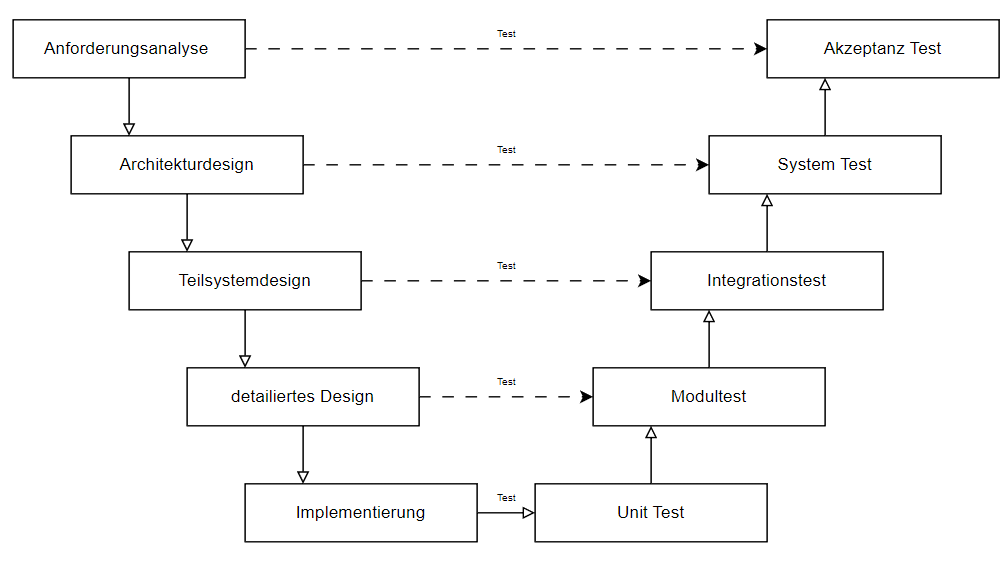
\includegraphics[width=\textwidth,height=\textheight,keepaspectratio]{img/vmodell}
    \caption{Softwareentwicklung und Test-Levels im V-Modell \cite[vgl. Figure 1.2]{software-testing}}
    \label{vmodelltest}
\end{figure}

Die verschiedenen Testebenen sollten schon im Designprozess Beachtung finden, denn die Formulierung von Test kann dabei helfen Designfehler zu finden
noch bevor die Software entwickelt wird~\cite[vgl. 1.1.1].
Die verschiedenen Ebenen der Tests spiegeln auch verschiedene Ansichten in den Tests wieder.
\newpage
\begin{figure}[h!]
    \begin{description}
        \item[Akeptanz Test] - Betrachten der Software hinsichtlich der Anforderungen
        \item[System Test] - Betrachten der Software hinsichtlich der Architektur
        \item[Integrationstest] - Betrachten der Software hinsichtlich der Teilsysteme
        \item[Modultest] - Betrachten der Software hinsichtlich detaiiliertem Design
        \item[Unit Test] - Betrachten der Software hinsichtlich konrekter Implementierung
    \end{description}\cite[vgl. 1.1.1]{software-testing}
\end{figure}

Im folgenden gehen wir noch einmal kurz auf jede einzelne Testebene etwas präziser ein.
Dabei ist die Reihenfolge von feingranular zu grobgranular.


\subsubsection{Unit Test}

Als feingranularste Testbene ist das Ziel des Unit-Testings den entwickelten Code zu testen.
Eine einzelne $Unit$ ist in Objekt-Orientierter Programmierung eine Funktion oder Methode~\cite[vgl. Unit Testing]{software-testing-craftmans}.
Ein einzelner Unit Test konzentriert sich dabei auf eine Funktion oder Methode.

\begin{figure}[h!]
    \begin{lstlisting}[language=Python]
        def add(a, b):
            return a + b
    \end{lstlisting}
    \caption{Eine einfache Python-Funktion}
    \label{unitfkt}
\end{figure}

\begin{figure}[h!]
    \begin{lstlisting}[language=Python]
    def test_add_positive():
        self.assertEqual(add(3, 5), 8)

    def test_add_negative():
        self.assertEqual(add(-3, -5), -8)

    def test_add_mixed():
        self.assertEqual(add(5, -3), 2)
    \end{lstlisting}
    \caption{Drei Unit Tests für die add-Funktion}
    \label{unitfkttest}
\end{figure}

Er prüft, ob die gegebene Einheit bei bekannten Eingaben die erwarteten Ausgaben liefert.
Für diese Tests werden häufig Testframeworks genutzt die bei der Entwicklung und Ausführung der Tests helfen~\cite{software-testing}.
In Abbildung~\ref{unitfkt} wurde eine Funktion defineirt und in Abbildung~\ref{unitfkttest} sind drei UnitTest mit PyTest~\cite{pytest} definiert.
Die Tests führen verschiedene Methoden aus und prüfen, dass das Ergebnis mit der Erwartung übereinstimmt.
Das $assertEqual$ übernimmt dabei die Auswertung.

\subsubsection{Modul Test}

Eine Granularitätsebene höher ist das Modul Testen.
Ein Modul ist eine Sammlung von Units~\cite[vgl. S. 6]{software-testing}.
Ziel ist es, die Interoperabilität der einzelnen Units in einem Modul sicherzustellen~\cite[vgl. S. 6]{software-testing}.

\begin{figure}[h!]
    \begin{lstlisting}[language=Python]
        def add(a, b):
            return a + b
        def sub(a, b):
            return a - b
        def mul(a, b):
            return a * b
        def quo(a, b):
            return a / b
    \end{lstlisting}
    \caption{Eine Python Rechenmodul}
    \label{modul}
\end{figure}

Ein Modul wird nun getestet, indem geprüft wird, dass die einzelnen Funktionen untereinander richtig miteinander interagieren.

\begin{figure}[h!]
    \begin{lstlisting}[language=Python]
    def test_rechenmodul():
        testResult = (mul(add(2,3), sub(3,2)))
        self.assertEqual(testResult, 5)
    \end{lstlisting}
    \caption{Eine Modul Test}
    \label{modultest}
\end{figure}

Anzumerken ist jedoch, dass die Interoperabilität im Modul-Test nur innerhalb eines Moduls getestet wird~\cite[vgl. S. 6]{software-testing}.

\subsubsection{Integrations Test}

Das Integrationstesten übernimmt das Testen von Interoperabilität zwischen verschiedenen Modulen~\cite[vgl. S. 7]{software-testing}.
Es wird dabei davon ausgegangen, dass die einzelnen Module zuvor korrekt getestet worden sind und die einzelnen Module korrekt arbeiten~\cite[vgl. S. 7]{software-testing}.
Testobjekt sind vor allem die Schnittstellen der einzelnen Module und damit auch die Kommunikation zwischen den Modulen.

\begin{figure}[h!]
    \begin{lstlisting}[language=Python]
def nnwUser(name, gb, email):
    pw = generateRandomPw()
    return new User(name, gb, email, pw)
    \end{lstlisting}
    \caption{Modul 1}
    \label{modul1}
\end{figure}

\begin{figure}[h!]
    \begin{lstlisting}[language=Python]
def saveUser(User user):
    db.save(user)
def getUser(name):
    db.findUser(name)
    \end{lstlisting}
    \caption{Modul 2}
    \label{modul2}
\end{figure}

Ein Integrationstest für beide Module wäre nun, zu testen, ob ein neu angelegter Nutzer ordentlich gespeichert wird und ob dabei die zugewiesenen Daten
auch passend bleiben.

\begin{figure}[h!]
    \begin{lstlisting}[language=Python]
def testAddNewUserAndSaveUserAndGetUser():
        user = newUser("Peter", "01.04.1980", "p@test.de")
        saveUser(user)
        self.assertEqual(getUser("Peter"), user)
    \end{lstlisting}
    \caption{Integrationstest zwischen Modul 1 und Modul 2}
    \label{integtest}
\end{figure}

Im Kontext dieser Arbeit werden wir untersuchen, wie solche Tests automatisiert für GraphQL erstellt werden können.
Hinter jedem verschiedenen Typen von GraphQL steckt ein Resolver, welcher als ein eigenes Modul gesehen werden kann.
Die Interoperabilität dieser Module gilt es im folgenden dann automatisiert zu testen.

\subsubsection{System Test}

Um zu testen, ob nun nicht nur einzelne Teile des Systems gut miteinander funktionieren, sondern auch das ganze System als
solches, nutzt man die System-Tests~\cite[vgl. S. 6]{software-testing}.
Die Tests werden auf Grundlage der Spezifikation des Systems erstellt.
Es wird davon ausgegangen, dass die einzelnen Module hier wie erwartet funktionieren.
Im Vordergrund dieser Testebene steht, dass die Software die Spezifikation, also die Erwartungen an sich, erfüllt.

\subsubsection{Akzeptanz Test}

Die finale Ebene des Testprozesses ist der Akzeptanz Test.
In dieser Ebene wird die Software aus Sicht des Endnutzers geprüft, oft ist der Endnutzer auch Teil dieses Prozesses~\cite[vgl. S.6]{software-testing}.
Ziel ist es, zu verifizieren, dass die Analyse und Umsetzung des Problems erfolgreich ist und der Nutzer mit der entwickelten Lösung
zufrieden ist~\cite[vgl. S.6]{software-testing}.

\subsection{Testabdeckung}

Wir kennen nun verschiedene Ebenen und Sichtweisen des Testens.
Allerdings ist noch nicht klar, wann ausreichend getestet wurde und ob wir überhaupt genügend testen können.
Hier zu nutzen wir formale Abdeckungskriterien wie sie in~\cite{software-testing} eingeführt werden.
Sie helfen uns, sinnvolle Testfälle zu entwickeln und zu entscheiden, wann ausreichend getestet wurde.
Sollte man nämlich davon ausgehen, dass man einfach alle möglichen Eingaben an eine Funktion testen kann, so kommt
man sehr schnell an die Erkentniss, dass dies unmöglich ist.
Als Beispiel sei hier eine simple Addition von 2 64-bit Integer genannt.
Für eine komplette Testung dieser simplen Addition gibt es \verb+2^64 ≈ 18 Trillionen+ Kombinationen.
Mit einem 3GHz Prozessor wäre eine vollständige Testung nach \\ 2^{64} / 3.000.000.000 $ \approx $ 6.149.571 Sekunden (69 Tage) erledigt.
Betrachten wir weiterhin einen Java-Compiler so ist der Eingaberaum von Programmen die zum Test stehen effektiv unendlich und somit nicht testbar \cite[vgl. 1.3 Coverage Criteria for Testing]{software-testing}.

\subsubsection{Abdeckungskriterien}

Wie gezeigt ist ein "vollständiges Testen" - also ein ausprobieren aller Möglichkeiten einfach unmöglich.
Hierdurch sind wir gezwungen einen anderen Ansatz zu verfolgen.
Abdeckungskriterien liefern hierbei einen Ansatz, die einem dabei helfen können, sinnvolle Tests zu entwickeln und zu entscheiden, wann genug Tests entwickelt wurden.
Im folgenden sehen wir die Abdeckungskriterien auch als Testanforderungen~\cite[vgl. 1.3 Coverage Criteria for Testing]{software-testing}

\begin{definition}
    Eine Testanforderung ist ein spezifisches Element eines Softwareartifkates das einen Testfall erfüllen muss.~\cite[Def. 1.20]{software-testing}
\end{definition}

Dabei soll ein Abdeckungskriterium erfüllt sein, wenn alle seine Testanforderungen erfüllt sind.

\begin{definition}
    Ein Abdeckungskriterium ist eine Regel oder eine Sammlung von Regeln, die Testanforderungen an eine Menge von Testfällen stellen~\cite[Def. 1.21]{software-testing}
\end{definition}

Um zu messen, wie gut ein Abdeckungskriterium durch eine Menge an Tests umgesetzt wird, führen wir die Abdeckung ein.
Einerseits ist es manchmal sehr schwierig ein Abdeckungskriterium vollständig zu erreichen, andererseits können
wir so messen, ob das Kriterium erfüllt wurde~\cite[vgl. S. 18]{software-testing}.

\begin{definition}
    Gegeben sei eine Menge an Testanforderungen $TR$ für ein Abdeckungskriterium $C$. 
    Eine Menge an Testfällen $T$ erfüllt $C$ wenn gilt, 
    dass für jede Testanforderung mindestens ein Test existiert der diese Testanforderung erfüllt.~\cite[vgl. Def. 1.22]{software-testing}
\end{definition}

Es gibt diverse Abdeckungskriterien die auf verschiedenen Annahmen beruhen.
Ist das Ziel, dass alle Entscheidungen in einem Programm abgedeckt sein soll (Branch-Coverage), so führt jede Entscheidung zu zwei
Testanforderungen, eine Anforderung für den positiven und eine für den negativen Entscheidungsfall~\cite[vgl. S. 17]{software-testing}.
Soll jede Methode mindestens einmal aufgerufen werden (Call-Coverage), so führt jede Methode zu einer Testanforderung um diese Methode abzudecken~\cite[vgl. S. 17]{software-testing}
Im folgenden Kapitel~\ref{graphueberdeckung} konzentrieren wir uns auf Abdeckungskriterien für Graphen.